\newpage
\part{Rendu}
    Après avoir détecter le tag dans l'image, la seconde grande étape est de projeter un modèle 3D sur la scène. Pour cela, l'utilisateur indique au lancement du programme le ou les modèles à utiliser, avec ou non des matériaux, et ceux-ci seront rendus à chaque image.

    \section{Gestion des objets}

        \subsection{Objets}

            \subsubsection{Définition du format}                
                Un objet 3D est composé de sommets, formant des faces d'au moins 3 côtés. Le format le plus simple pour stocker un modèle 3D est le \emph{.obj}. Cette norme définie les sommets, les matériaux et les normales pour chaque face dans un format texte. Chaque ligne début par un indicateur puis les valeurs à proprement parler. Un exemple est visible figure \ref{fig:obj}. Nous utilisons 4 indicateurs :
                \begin{itemize}
                    \item v x y z : sommet à la position $(x, y, z)$
                    \item vt u v [z] : coordonnées de texture (voir partie \ref{subsubsec:materiaux})
                    \item vn x y z : normale (voir partie \ref{subsubsec:lumiere})
                    \item f v/vt/vn [...] : les faces de l'objet avec un triplet pour chaque sommet (minimum 3). La coordonnée de texture peut être vide (v//vn).
                \end{itemize}
                
                \begin{figure}[h]
                    \centering
                    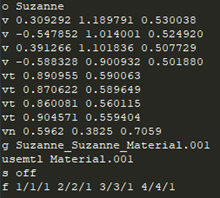
\includegraphics[scale=0.8]{img/rendu/obj.png}
                    \caption{Exemple de fichier \emph{.obj}}
                    \label{fig:obj}
                \end{figure}
                Nous avons écrit un parser afin de décomposer ce fichier \emph{.obj}.

                Chaque objet est contenu dans une classe \emph{Object}. Celle-ci contient un ensemble de face qui correspond à plusieurs points, une couleur et une normale. Plusieurs fonctions sont également disponible afin de manipuler l'objet : \emph{rotate}, \emph{scale}, \emph{position}\dots

            \subsubsection{Matériaux}
            \label{subsubsec:materiaux}

            Afin de rendre les objets plus agréables à l'\oe il, nous avons décider d'implémenter la gestion des matériaux. Nous utilisions déjà le format \emph{.obj} pour les modèles, il semblait donc naturel d'utiliser les \emph{.mtl}, format défini par la même norme, pour les matériaux. 

            Un fichier \emph{.mtl} est un fichier texte, et nous utilisons uniquement une seule ligne de ce fichier, \emph{map\_kD}, qui indique le nom de l'image texture utilisée. Les coordonnées de texture renseignées dans le \emph{.obj} indiquent des pourcentage dans cette image, respectivement la largeur et la hauteur. Nous travaillons ici avec des images 2D.

            \begin{figure}[h]
                \centering
                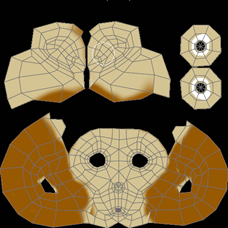
\includegraphics[scale=0.8]{img/rendu/texture.png}
                \caption{Texture découpée par face}
                \label{fig:texture}
            \end{figure}

            Dans la figure \ref{fig:texture}, nous pouvons voir les faces en fonction des coordonnées indiquées pour chaque sommet. Afin de pouvoir utiliser cette texture, il faut déformer le polygone pour l'appliquer sur le polygone projeté. Cependant, cette étape est très coûteuse en performance car il faut l'appliquer pour chaque polygone de chaque objet à chaque image de la vidéo. Nous avons alors choisi de préférer le temps réel et, pour cela, une face ne possède qu'une seule couleur, inscrite directement dans la classe \emph{Object}. Pour choisir la couleur, nous prenons simplement la couleur du pixel au centre du polygone sur l'image texture. Cela nous donne alors un objet avec des flat color. 
            
            Une amélioration possible du programme pourrait être de prendre en compte les autres paramètres du fichier \emph{.mtl} et donc de ne pas obligatoirement utiliser d'image pour la texture.

        \subsection{Scène}

            La scène est un regroupement de tous les objets ainsi que de la caméra. Afin de rendre donner une liberté à l'utilisateur et de ne pas recompiler à chaque fois le programme, nous avons défini un format CSV \emph{.scene} (figure \ref{fig:scene}) qui défini chaque objet de la scène ainsi que leur position et leur rotation.

            \begin{figure}[h]
                \centering
                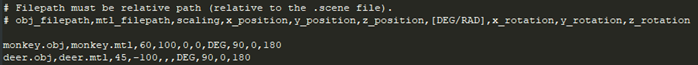
\includegraphics[scale=0.8]{img/rendu/scene.png}
                \caption{Fichier CSV \emph{.scene}}
                \label{fig:scene}
            \end{figure}

            Chaque champ est optionnel, à l'exception du premier qui défini l'objet à charger. Un champ vide prendra une valeur par défaut inscrite dans le code.

            Notre méthode pour le placement et l'échelle des objets à cependant un défaut. Il faut déterminer à la main la bonne position et la bonne échelle pour que l'objet soit visible et au bon endroit. En effet, deux logiciels de modélisation n'enregistre pas l'échelle de la même façon. Par exemple, avec Blender, une échelle entre 45 et 55 est idéale. Tous les \emph{.obj} fournis dans le projet ont été créés par nous-même sous Blender.

        \subsection{Lumière}
        \label{subsubsec:lumiere}

        Une méthode d'ombrage plat (\textit{Flat Shading}) a été implémentée afin de rendre l'apparence des objets plus réaliste.

        La lumière est représentée par un vecteur qui donne sa direction. Afin de déterminer l'éclairage d'une face, nous utilisons la normale définie dans le \emph{.obj}. Nous ne souhaitons qu'une seule illumination par face, nous calculons alors la moyenne des normales des sommets que nous enregistrons dans la face avec la couleur et les points. 

        % TODO: reprendre une autre image
        \begin{figure}[!h]
            \centering
            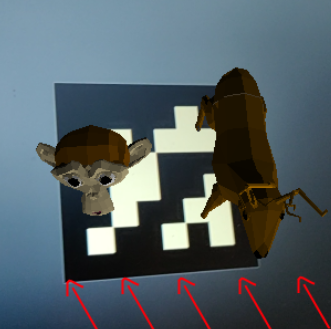
\includegraphics[scale=0.5]{img/rendu/flat_shading.png}
            \caption{Ombrage plat sur les objets à partir d'une source lumineuse représentée par les flèches rouges}
            \label{fig:lumiere}
        \end{figure}

        Ensuite, la luminosité est calculée pour chaque face en fonction de l'angle entre sa normale et la direction de la lumière. Plus l'angle est proche de 0°, plus les vecteurs sont alignés et donc plus la face est dans l'ombre. Inversement, plus l'angle est proche de 180°, plus la face est éclairée. Cet angle est normalisé puis multiplié à la couleur de la face. Nous pouvons voir cette effet, avec les matériaux, dans la figure \ref{fig:lumiere}. Le rendu sera expliqué dans la partie suivante.

    \section{Caméra et projection}
        Après avoir chargé les objets dans la scène 3D, il faut projeter ses objets sur l'image en fonction du tag. Nous utilisons cette relation :
        \begin{equation*}
            \begin{pmatrix}
                u \\ v \\ 1
            \end{pmatrix}
            = K.P.E.
            \begin{pmatrix}
                x_w \\ y_w \\ z_w \\ 1
            \end{pmatrix}
        \end{equation*}
        avec $u,v$ les coordonnées dans le plan image en pixels, $K.P$ les paramètres intrinsèques de la caméra, $E$ les rotations et translation de la caméra dans le repère monde et $x_w, y_w, z_w$ les coordonnées du point 3D dans le repère monde.

        \subsection{Calibration}
            Afin de déterminer les paramètres intrinsèques de la caméra, nous avons développé une fonction pour les calculer. Elle se base sur la prise de photos de checkerboard tel que la figure \ref{fig:checkerboard}.

            \begin{figure}[!h]
                \centering
                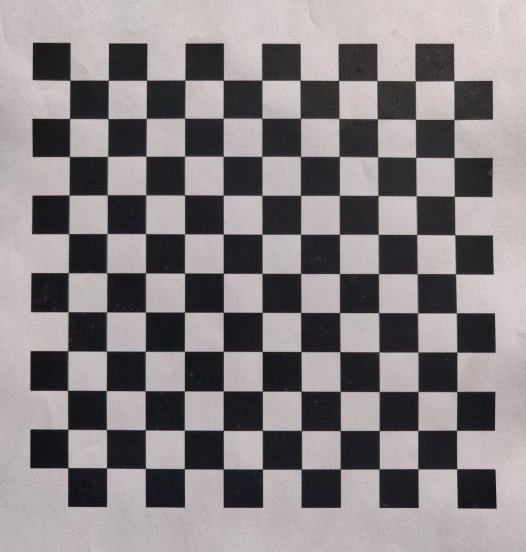
\includegraphics[scale=0.3]{img/rendu/checkerboard.jpg}
                \caption{Exemple de checkerboard}
                \label{fig:checkerboard}
            \end{figure}

            Des images de différents angles sont nécessaires. Après quelques essais, environ 5-6 images sont suffisantes pour estimer les paramètres. La méthode se base principalement sur la fonction \emph{cv::calibrateCamera} d'OpenCV. Elle prend en paramètres les coordonnées des points 3D et leur correspondance sur l'image (les points 2D). Étant donné que le checkerboard est connu, on peut donner des coordonnées à chaque coins des carrés en supposant que $z=0$, ces points étant sur le même plan. Les coins du checkerboard sur l'image peuvent être trouvés par la fonction \emph{cv::findChessboardCorners} d'OpenCV.

            Après avoir calculer les paramètres intrinsèques, nous les enregistrons dans un format texte avec l'extension \emph{.cam} (figure \ref{fig:cam})

            \begin{figure}[!h]
                \centering
                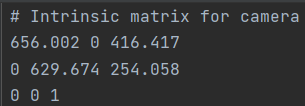
\includegraphics[scale=0.8]{img/rendu/cam.png}
                \caption{Fichier \emph{.cam} représentant les paramètres intrinsèques}
                \label{fig:cam}
            \end{figure}

            Ce fichier se compose d'une matrice 3x3 représentant les paramètres intrinsèques ainsi :
            \begin{equation*}
                \begin{pmatrix}
                    f_x & s & x_0 \\
                    0 & f_y & y_0 \\
                    0 & 0 & 1
                \end{pmatrix}
            \end{equation*}
            $f$ est la distance focale en pixels. Dans une caméra parfaite, $fx$ et $f_y$ sont égaux mais dans les faits, ils peuvent différés, ce qui cause des pixels non carrés. $s$ est une distortion de l'image, souvent égale à 0, ce qui est suffisant dans notre cas. Enfin $(x_0, y_0)$ est le centre optique de l'image, l'intersection entre l'axe optique et le plan image. Il est en général plus ou moins au centre de l'image. 

        \subsection{Projection}
        % TODO: expliquer l'extraction de z via l'homographie
        % TODO: algorithme du peintre
